% ************* Make changes after \begin{document} ***************
%
%  August 07: original template is from 
%  http://www.slac.stanford.edu/econf/editors/eprint-template/instructions.html
%             Modified for CHARM 2007
%
%% ****** Start of file slactemplate.tex ****** %
%%
%%
%%   This file is part of the APS files in the REVTeX 4 distribution.
%%   Version 4.0 of REVTeX, August 2001
%%
%%
%%   Copyright (c) 2001 The American Physical Society.
%%
%%   See the REVTeX 4 README file for restrictions and more information.
%%
%
% This is a template for producing manuscripts for use with REVTEX 4.0
% Copy this file to another name and then work on that file.
% That way, you always have this original template file to use.
%
\documentclass[twocolumn,twoside,slac_two]{revtex4}
\usepackage{graphicx}
\usepackage{fancyhdr}
\pagestyle{fancy}
\fancyhead{} % clear all fields
\fancyhead[C]{\it {
Proceedings of the DPF-2009 Conference, Detroit, MI, July 27-31, 2009
}} \fancyhead[RO,LE]{\thepage}
\fancyfoot{} % clear all fields
\fancyfoot[LE,LO]{}

\renewcommand{\headrulewidth}{0pt}
\renewcommand{\footrulewidth}{0pt}
\renewcommand{\sfdefault}{phv}

\setlength{\textheight}{235mm}
\setlength{\textwidth}{170mm}
\setlength{\topmargin}{1mm}

\bibliographystyle{apsrev}

% ************* Make changes after here  ***************

\begin{document}

%Title of paper
\title{Alignment of the CMS Muon System with Tracks}

% Repeat the \author .. \affiliation  etc. as needed
%
% \affiliation command applies to all authors since the last
% \affiliation command. The \affiliation command should follow the
% other information

\author{J. Pivarski}
\affiliation{Department of Physics, Texas A\&M University 77843, USA}
\affiliation{The CMS Collaboration}
%
%

\begin{abstract}
As its name suggests, the Compact Muon Solenoid (CMS) features a full
tracking spectrometer for identifying and measuring the momenta of
muons. Every muon passes through 18--44 layers, providing a highly
redundant track capable of validating and improving the momentum
measurement from the CMS silicon tracker. But like any tracking
system, its performance depends on precise knowledge of the positions
of the tracking elements relative to one another and relative to the
tracker. We present methods to align the muon system with tracks and
the performance of these algorithms using cosmic rays and beam-halo
data from the 2008 run of the LHC.
\end{abstract}

%\maketitle must follow title, authors, abstract
\maketitle

\thispagestyle{fancy}

% body of paper here - Use proper section commands
% References should be done using the \cite, \ref, and \label commands
% Put \label in argument of \section for cross-referencing
%\section{\label{}}

%%%%%%%%%%%%%%%%%%%%%%%%%%%%%%%%%%
\section{Introduction}

The Compact Muon Solenoid (CMS) experiment~\cite{cms} is designed to
explore physics at the TeV energy scale, exploiting proton-proton
collisions delivered by the Large Hadron Collider (LHC)~\cite{lhc}.
Muons provide a particularly useful probe of new phenomena, in that
many signatures of new physics and few QCD-related backgrounds yield
energetic muons.  A primary component of the CMS design, therefore, is
a large muon tracking system with excellent muon efficiency and
background rejection~\cite{mutdr}.

Data from the muon system also contribute to the muon momentum
resolution, particularly for the most energetic muons.  The
trajectories of highly energetic muons have small curvature in the
magnetic field, and the large distance of muon detectors from the LHC
beamline (up to 7~m) help to resolve the curvature, and therefore the
transverse momentum ($p_T$) of the muons.  However, the spatial
resolution on which this momentum measurement depends requires the
locations of muon system components to be well known; in other words,
the muon system must be well aligned.  The relevance of muon system
alignment for a sample physics signature ($Z' \to \mu\mu$) is
illustrated in Fig.~\ref{misaligned_spectra}.

\begin{figure}
\centering
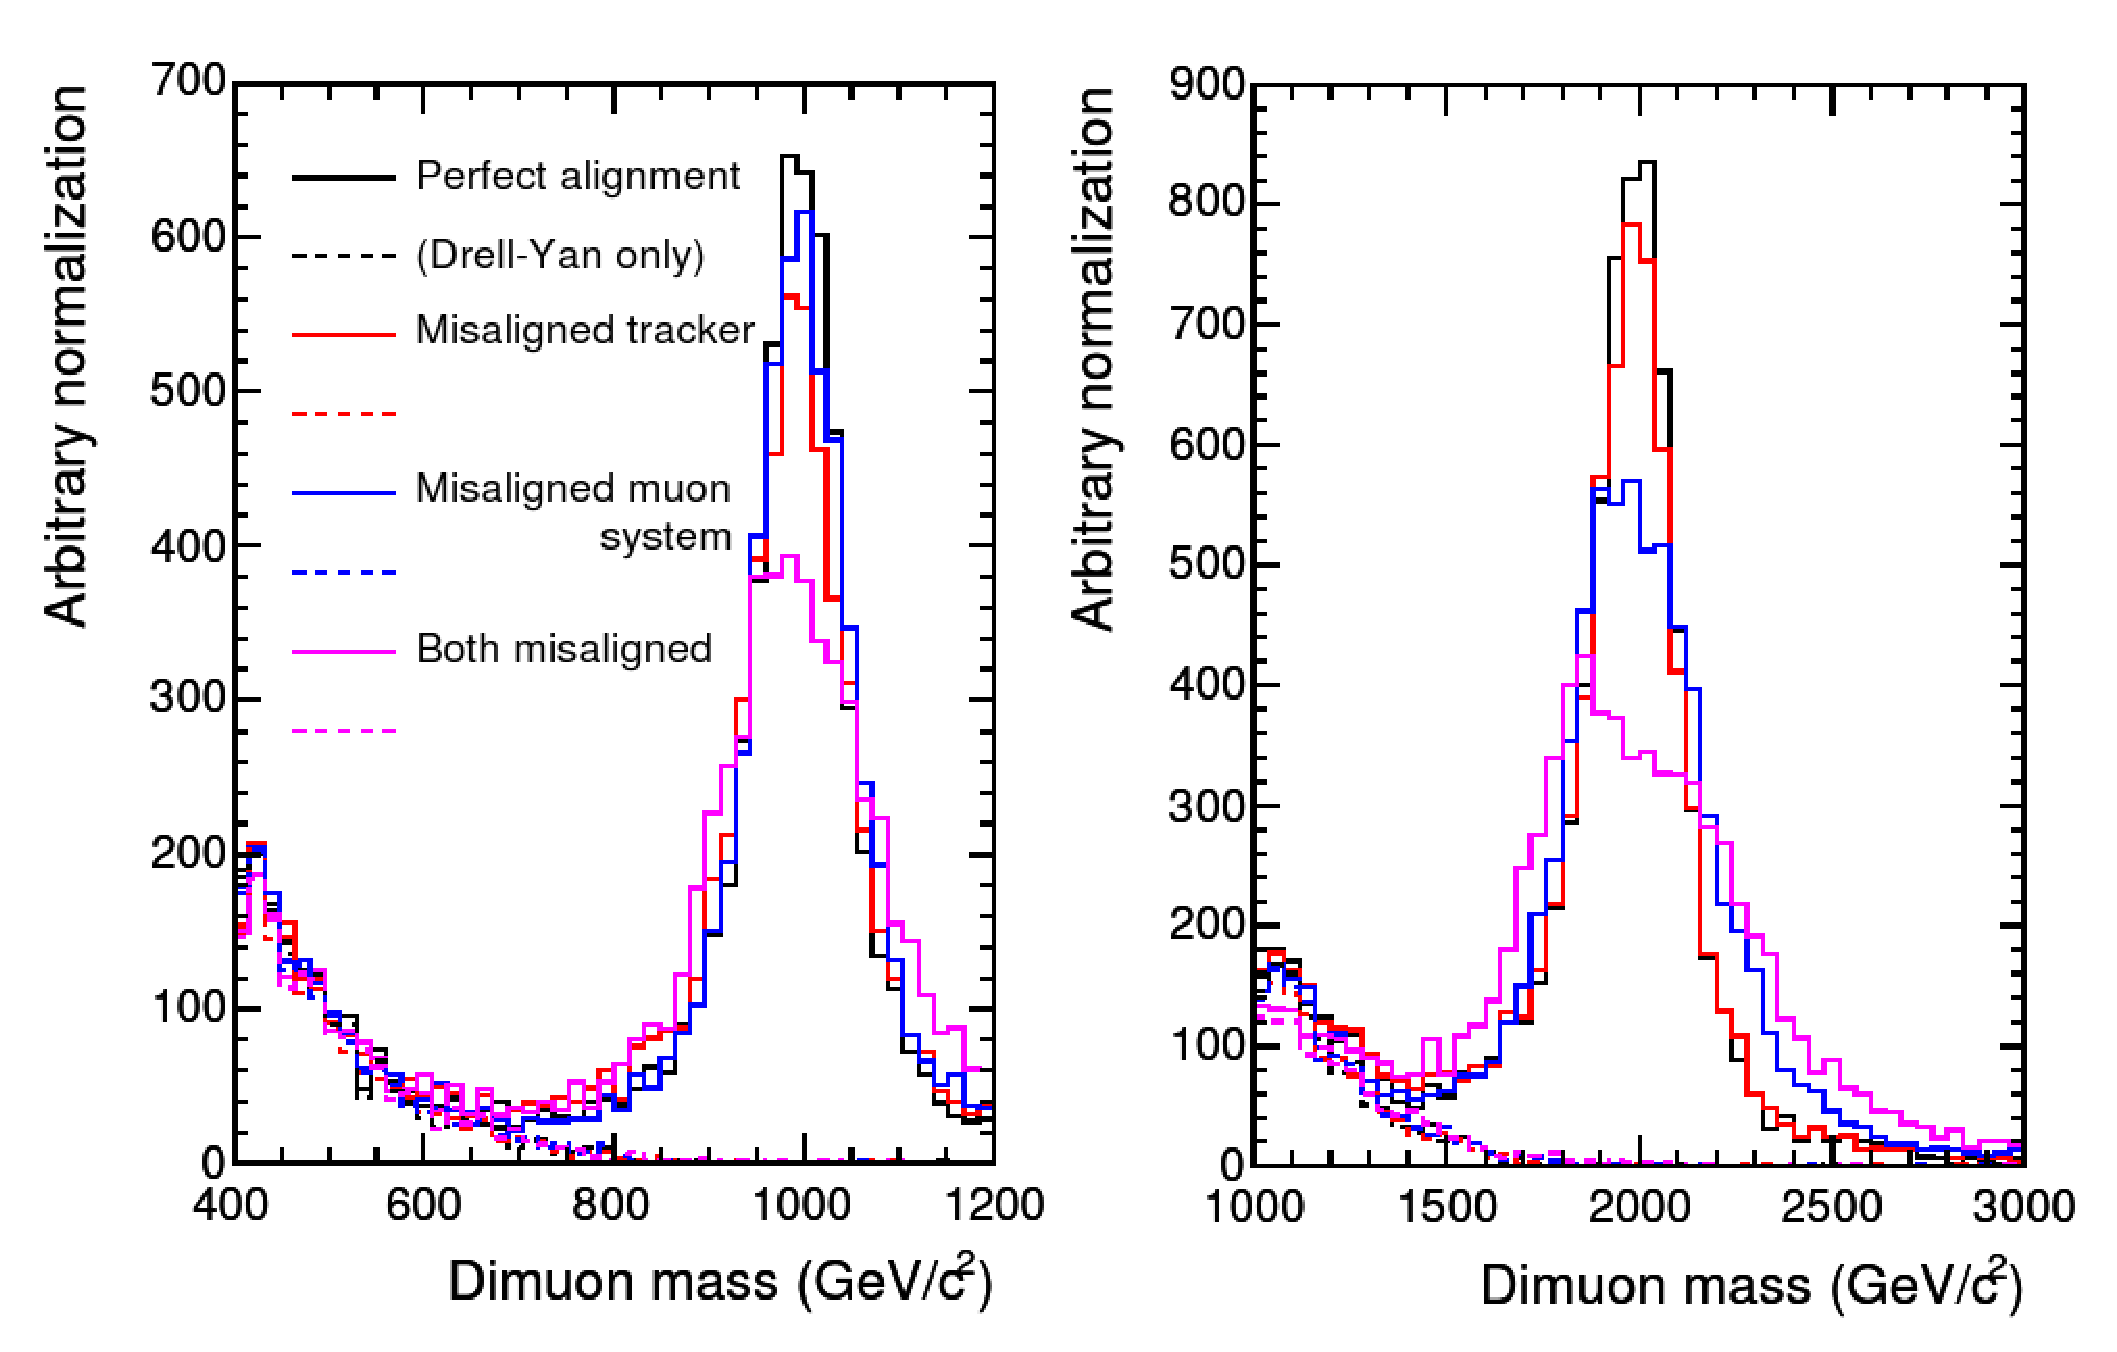
\includegraphics[width=\linewidth]{misaligned_spectra.eps}
\caption{Reconstructed dimuon mass for hypothetical 1~TeV (left) and
  2~TeV (right) $Z'$ bosons, under different assumptions of tracker
  and muon system misalignment.} \label{misaligned_spectra}
\end{figure}

The muon system is composed of hundreds of modular tracking chambers,
each containing 6--12 measurement layers.  Drift tube (DT) chambers
are arranged in a barrel geometry around the beamline, while Cathode
Strip Chambers (CSC) are oriented in endcap rings on both sides of the
collision point.  Muons traversing each chamber are reconstructed as
linear track segments, and these are combined with tracks in the
central CMS silicon tracker to form global muon tracks which span the
entire detector.

Alignment techniques have been developed to determine the positions
and orientations of the muon chambers by correcting systematic biases
in the distributions of tracks and local track segments.  While
these techniques were designed primarily for alignment using muons
from proton collisions, they have been successfully applied to cosmic
rays and beam-halo muons from the 2008 LHC beam circulation tests (see
Fig.~\ref{illustration}).

This paper presents the techniques and their results using
pre-collisions data.  The technique described in the
Section~\ref{sec:one} aligns each chamber relative to the CMS tracker
using tracker tracks, and it is demonstrated using cosmic rays
that traverse the muon barrel and the tracker.  Section~\ref{sec:two}
presents a technique for aligning CSC chambers within endcap rings
with much smaller event samples, and it is demonstrated using muons
from a 9-minute single-beam run of the LHC.

\begin{figure}
\centering

\includegraphics[width=0.47\linewidth]{CMS_exploded_barrel.eps}

\includegraphics[width=0.47\linewidth]{CMS_exploded_endcap.eps}
\caption{Illustration of the CMS detector, highlighting the barrel (left) and the endcap (right).  Cosmic ray muons are better probes of barrel alignment and beam-halo muons are better probes of endcap alignment due to the orthogonality to the respective detector measurement planes.} \label{illustration}
\end{figure}

%%%%%%%%%%%%%%%%%%%%%%%%%%%%%%%%%%
\section{Alignment relative to the CMS tracker with cosmic rays}
\label{sec:one}

The purpose of this procedure is to align all muon chambers in the
same coordinate system as the CMS tracker.  It will be used with
collisions muons when large samples become available (tens of inverse
picobarns), but cosmic ray datasets already collected have equivalent
sample sizes for the top and bottom chambers of the central barrel of
the muon system.

%%%%%%%%%%%%%%%%%%%%%%%%%%%%%%%%%%
\subsection{Method}

The basic idea is to use tracks from the CMS tracker as a reference to
position and orient each muon chamber.  For this procedure, track
parameters are determined using the tracker-only and are propagated
through the magnetic field map and material distribution to the muon
chambers, where they can be compared with the muon hits.
Figure~\ref{hip_explanation} illustrates the effect of a simple
displacement in chamber position, in which muon measurements (hits) are
offset from the extrapolated track.  In a large sample, the
distribution of residuals (hits minus track intersections with the
measurement layers) has a systematic bias which can be inverted to
derive and correct the misalignment.

\begin{figure}
\centering
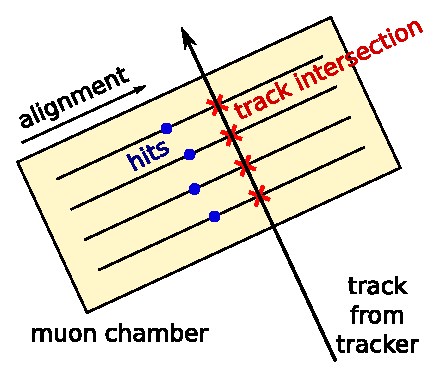
\includegraphics[width=0.5\linewidth]{hip_explanation.eps}
\caption{Cartoon of a misaligned muon chamber: misalignment is inferred from a systematic bias in the hits-minus-track intersection distribution.} \label{hip_explanation}
\end{figure}

In general, six rigid-body alignment parameters--- three translations
and three rotations--- must be determined from four component muon
chamber residuals, two displacements ($x$ and $y$) and two angles
($\frac{dx}{dz}$ and $\frac{dy}{dz}$); see Fig.~\ref{dt_coordinates}.
Estimators for the alignment corrections are derived from a residuals
dataset through the Jacobian of the transformation between the
4-dimensional residuals space and the 6-dimensional alignment
correction space: a 6$\times$4 matrix.  Additional corrections for
known propagation effects and potential magnetic field errors
generalize the linear problem into one that can be solved by a
non-linear fit.  A sample fit result is presented in
Figs.~\ref{exampleData_wh0st1sec10_MC}~and~\ref{exampleData_wh0st1sec10}.

\begin{figure}
\centering
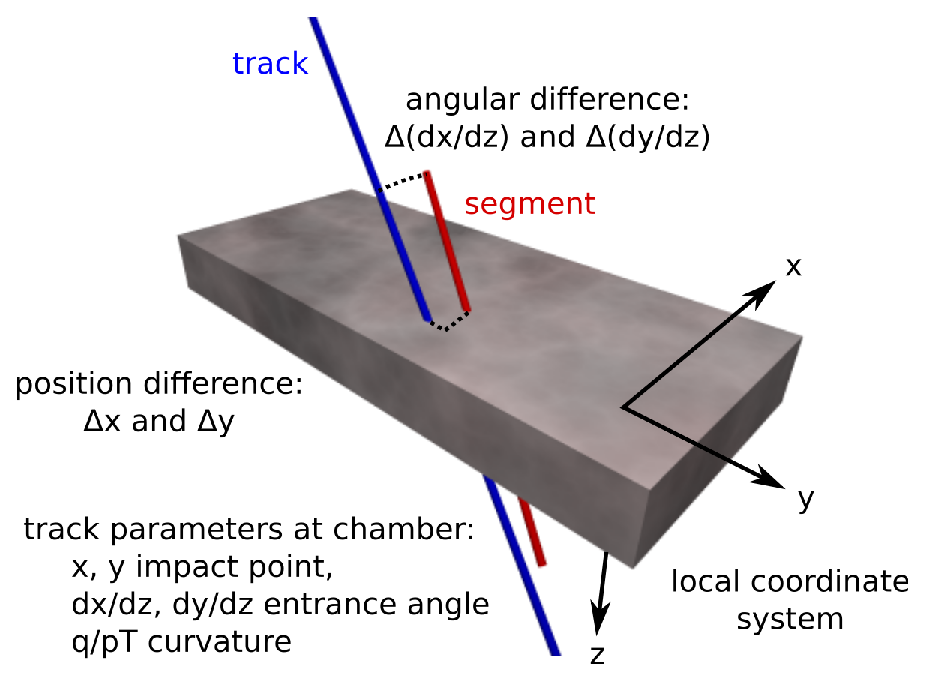
\includegraphics[width=\linewidth]{dt_coordinates.eps}
\caption{Definition of coordinates and 4-component residuals (two displacements and two angles).} \label{dt_coordinates}
\end{figure}

\begin{figure*}[p]
\centering
\begin{tabular}{p{0.47\linewidth} c p{0.47\linewidth}}
\begin{center}Before alignment (simulation)\end{center} & & \begin{center}After alignment (simulation)\end{center} \\
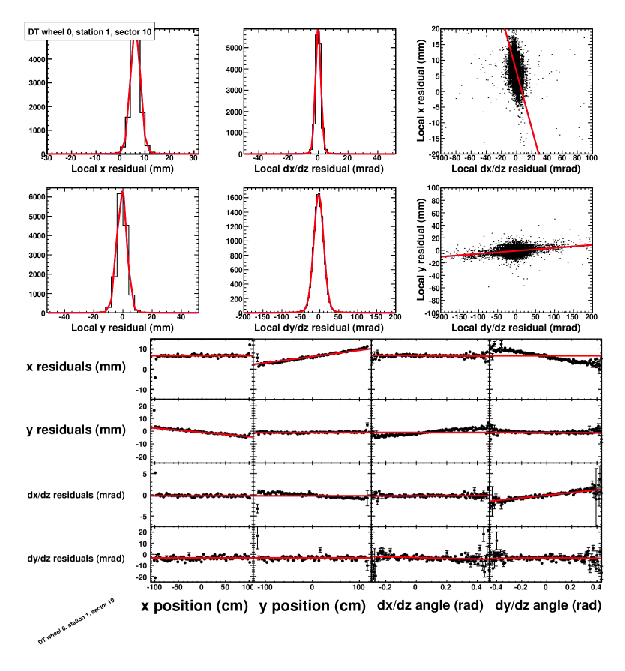
\includegraphics[width=\linewidth]{exampleMC_wh0st1sec10_before.eps} & &
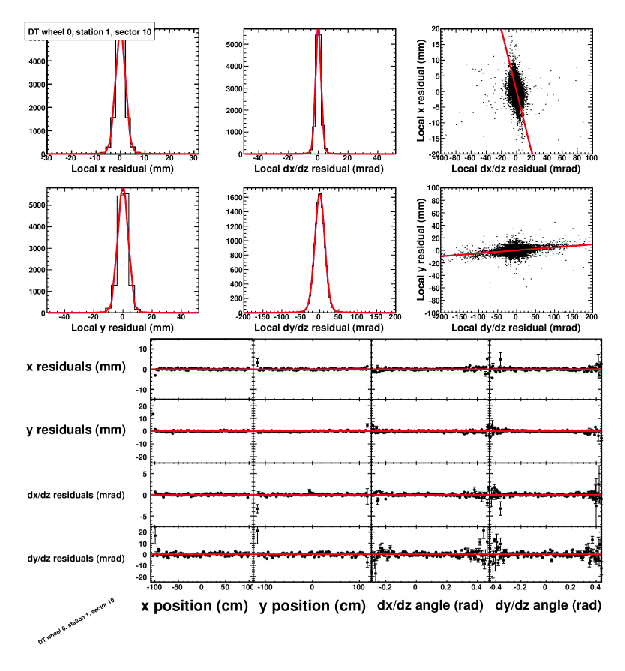
\includegraphics[width=\linewidth]{exampleMC_wh0st1sec10_after.eps}
\end{tabular}
\caption{Example alignment fit from {\bf simulated} cosmic rays (one chamber).  Left and right groups of plots are before and after alignment, respectively.  The six top histograms are each of the four residuals components and their correlations (detector effects).  The bottom 16 are residuals versus position and entrance angle (misalignment). \label{exampleData_wh0st1sec10_MC}}
\end{figure*}

\begin{figure*}[p]
\centering
\begin{tabular}{p{0.47\linewidth} c p{0.47\linewidth}}
\begin{center}Before alignment (data)\end{center} & & \begin{center}After alignment (data)\end{center} \\
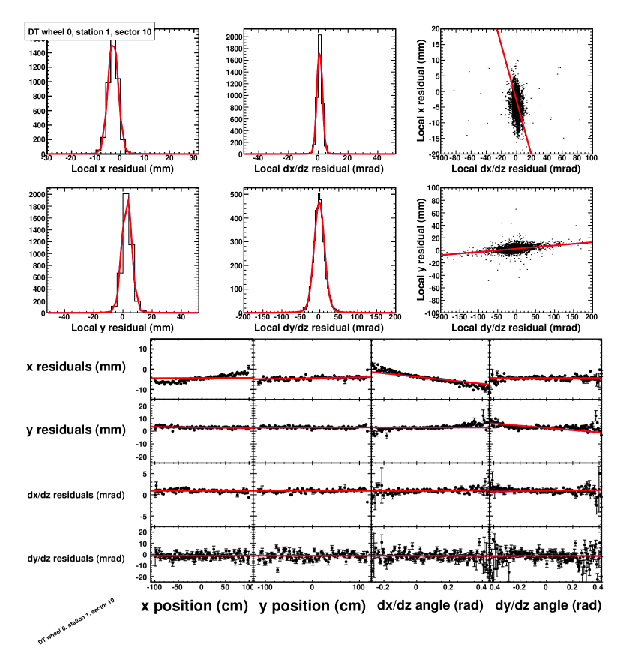
\includegraphics[width=\linewidth]{exampleData_wh0st1sec10_before.eps} & &
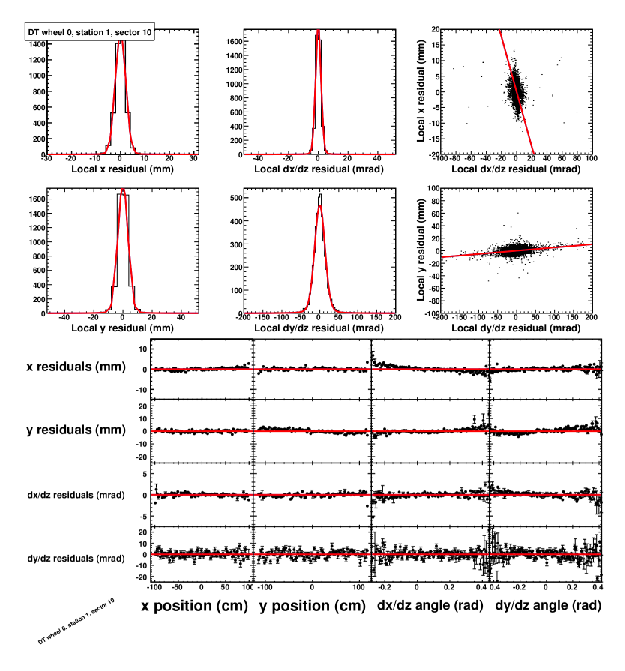
\includegraphics[width=\linewidth]{exampleData_wh0st1sec10_after.eps}
\end{tabular}
\caption{Example alignment fit from cosmic ray {\bf data}.  See Fig.~\ref{exampleData_wh0st1sec10_MC} caption for details. \label{exampleData_wh0st1sec10}}
\end{figure*}

Large numbers of cosmic rays passing through the tracker are only
available in the center of the barrel of the muon system.  Therefore,
the alignment was only applied using chambers from the central three
wheels (modular transverse cross-sections of the muon system),
excluding the two horizontal chambers on the left and right extremes
of each wheel.

%%%%%%%%%%%%%%%%%%%%%%%%%%%%%%%%%%
\subsection{Monte Carlo simulation}

To verify that the procedure is working, a cosmic ray Monte Carlo
sample was simulated with misaligned muon chambers.  The alignment
algorithm was applied to the simulated dataset and the real dataset
with the same parameters.  The simulation included all known detector
effects except for misalignment of the tracker, misalignment of layers
inside the chambers, and errors in the magnetic field map and material
budget, which can affect aligned chamber positions but do not test the
performance of the alignment algorithm itself.

Figure~\ref{hip_MC_simple2} presents the results of the test by
comparing each aligned chamber parameter with the true value, known in
simulation.  The local $x$ and $\phi_y$ coordinates determine the
bending of tracks in the transverse plane and hence set the momentum
scale.  Their accuracies, 200~$\mu$m and 0.1~mrad, respectively, are
approximately the scale of intrinsic hit resolutions
(100--300~$\mu$m), and hence residual misalignment does not dominate
the momentum resolution of high-energy muons.

\begin{figure*}
\centering
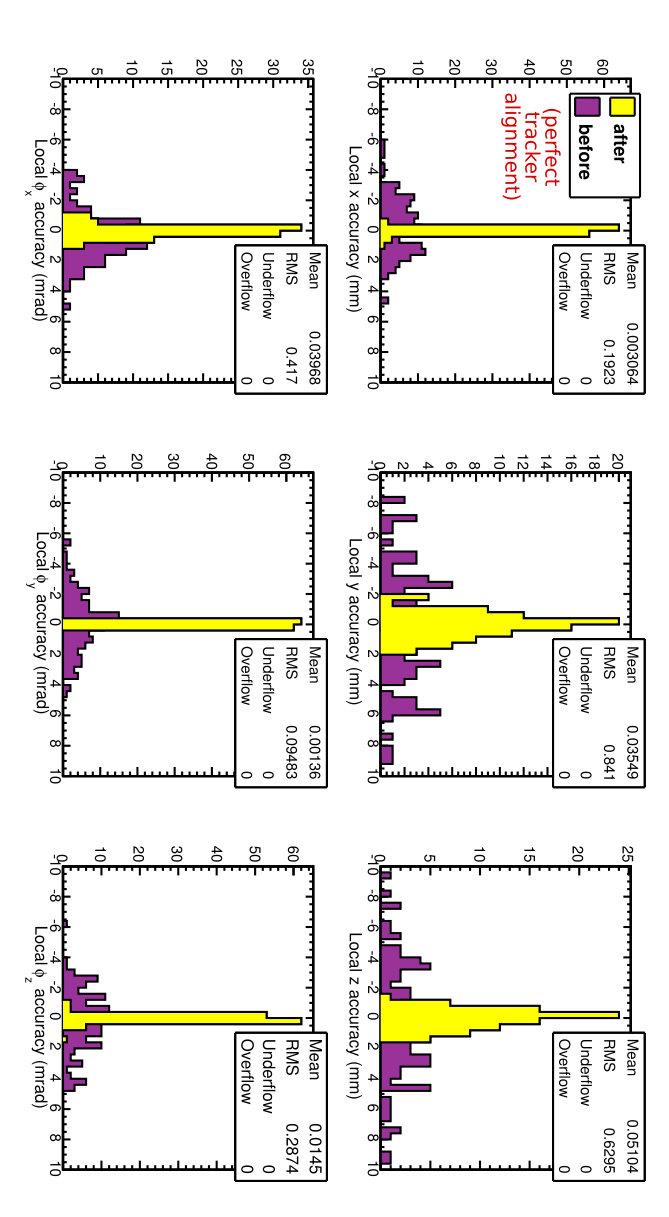
\includegraphics[height=\linewidth, angle=90]{hip_MC_simple2.eps}
\caption{Histogram of aligned chamber parameters minus true chamber parameters for a simulated cosmic ray alignment challenge.  To illustrate the performance of the alignment method itself, tracker misalignments were not considered.} \label{hip_MC_simple2}
\end{figure*}

%%%%%%%%%%%%%%%%%%%%%%%%%%%%%%%%%%
\subsection{Momentum resolution}

Optimization of momentum resolution is a primary goal of alignment,
but it can also serve as a cross-check.  To measure the momentum
resolution of tracks before and after muon chamber alignment, cosmic
rays traversing the entire CMS detector were split close to the
beamline and both halves were fitted independently.  Any differences
in track parameters between the top and bottom halves are purely
instrumental.

Figure~\ref{cosmic_splitting} presents the fractional curvature
resolution, that is, differences in curvature ($q/p_T$, where $q$ is
the muon charge) between the top and bottom cosmic ray tracks divided
by the curvature.  Cosmic rays were required to have $p_T >
200$~GeV/$c$ to increase sensitivity to muon misalignment.  Results
from several track-fitting procedures are presented: tracker-only (no
muon hits), tracker with first muon station hits (innermost chambers
only), before and after alignment.  Including only the first muon
station in track-fits reduces sensitivity to hit confusion from muon
showers, prominent for muons of several hundred GeV/$c$.  It also
limits this cross-check to test the alignment of the first muon
station.

\begin{figure*}
\centering
\mbox{ } \hfill 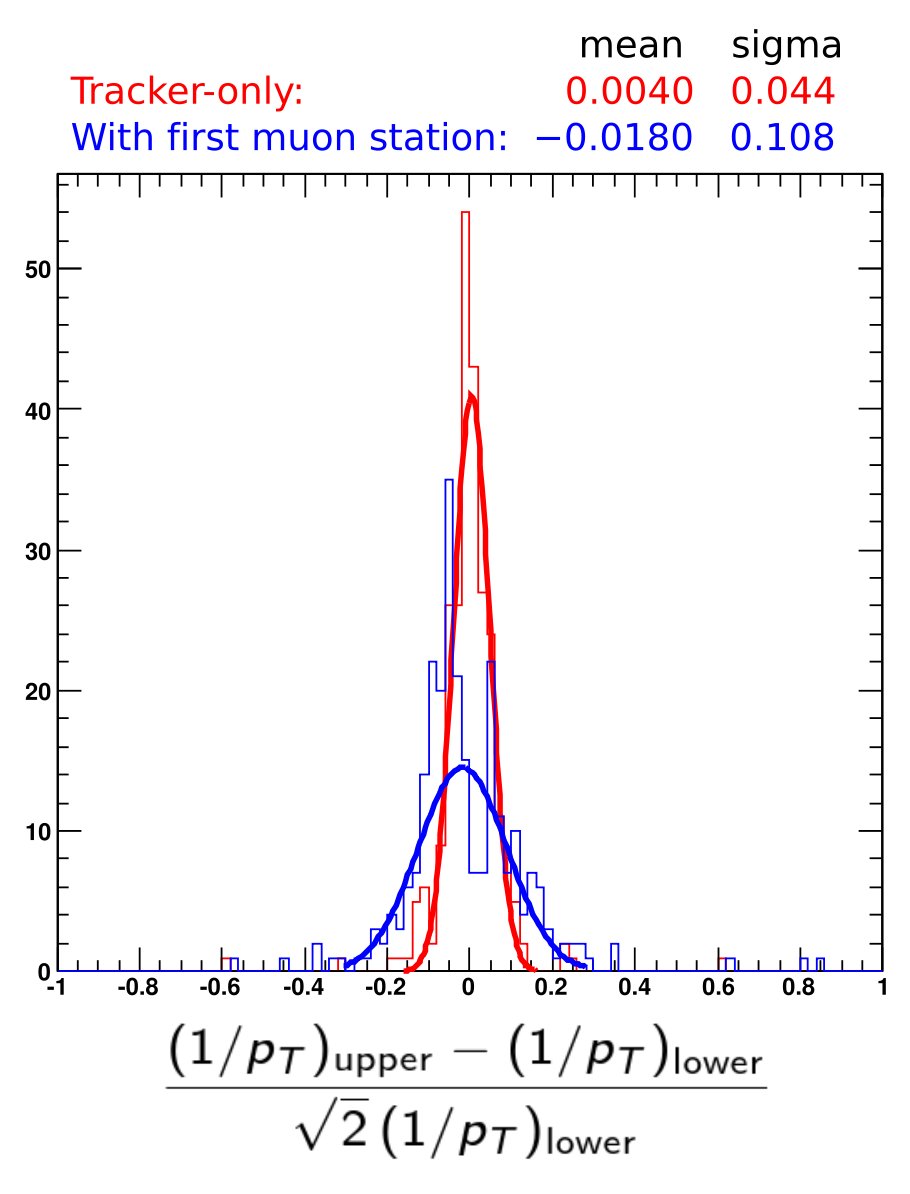
\includegraphics[width=0.35\linewidth]{without_alignment.eps} \hfill
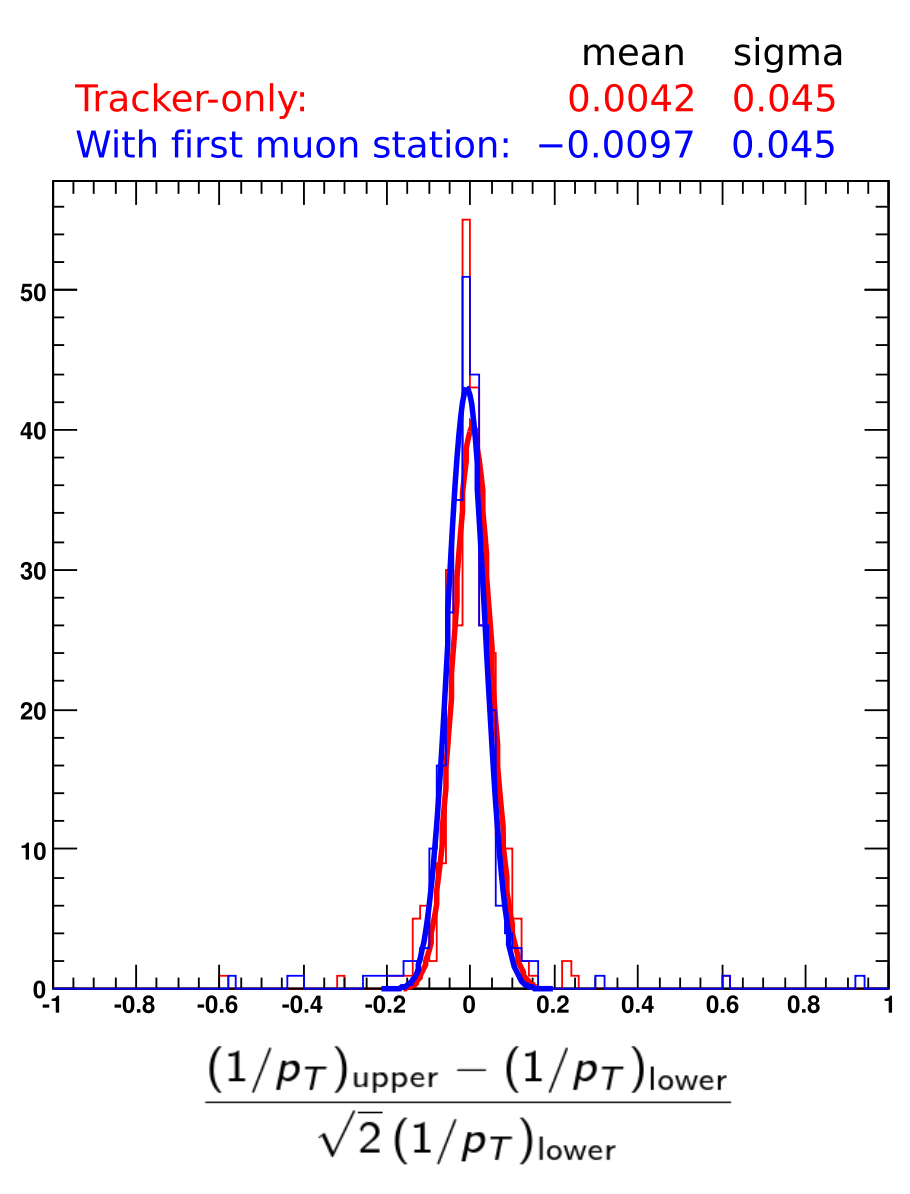
\includegraphics[width=0.35\linewidth]{with_alignment.eps} \hfill \mbox{ }
\caption{Curvature resolution for tracks ($p_T > 200$~GeV/$c$) including muon hits (blue) and not including muon hits (red), before alignment (left) and after alignment (right), derived from split cosmic ray tracks.} \label{cosmic_splitting}
\end{figure*}

For $p_T \approx 200$~GeV/$c$ muons, tracker hits dominate the
momentum resolution, but we can see the biasing effect of
misalignment.  Before alignment, track-fits including muon hits were
biased because hit positions were misreconstructed with small quoted
uncertainties (only the intrinsic hit uncertainties).  The bias
depends on which chambers the muons intersected, resulting in a
broadening of the whole distribution.  After alignment, the momentum
distribution is narrower and more centered, reproducing the resolution
of the tracker-only.  The tracker-only fits are unaffected by the muon
alignment, though the tracker-only distributions differ slightly
between the two cases because more muons were identified after muon
alignment.

%%%%%%%%%%%%%%%%%%%%%%%%%%%%%%%%%%
\section{Alignment of endcap rings with beam-halo muons}
\label{sec:two}

An alternate technique was used to align endcap CSC chambers using a
small number of beam-halo tracks from the LHC beam circulation tests
of 2008.

%%%%%%%%%%%%%%%%%%%%%%%%%%%%%%%%%%
\subsection{Method}

CSC chambers overlap along the edges of their active area, such that
muons passing through these overlap regions leave tracks in both
chambers in each pair (left of Fig.~\ref{overlaps_explantion}).
Uncertainties due to track propagation are negligible because the
tracks are not propagated through large amounts of material.  From the
continuity and linearity of observed tracks, one can derive the
relative positions of each pair of chambers, and propagate that
information transitively around rings of mutually-overlapping chambers
(right of Fig.~\ref{overlaps_explantion}).  The resulting measurement
is insensitive to the global position and orientation of each whole
ring, but precisely interaligns the chambers within the rings.

\begin{figure}
\centering
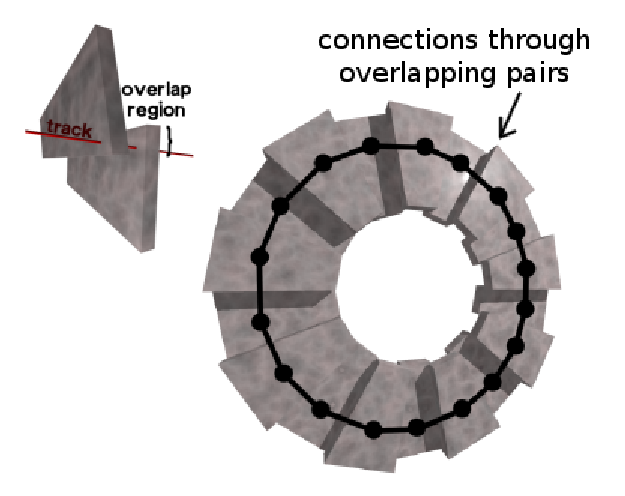
\includegraphics[width=0.8\linewidth]{matrix_description_onestation.eps}
\caption{The local CSC alignment algorithm uses track segments passing through pairs of neighboring chambers to determine relative alignments, and builds a ring geometry by combining pairwise information in a single fit.} \label{overlaps_explantion}
\end{figure}

Of the six rigid-body alignment parameters, this method is sensitive
to $r\phi$ (rotation around the nominal beamline), $\phi_z$ (rotation
in the measurement plane, which is perpendicular to the beamline), and
$\phi_y$ (rotation around radial axes).  These are illustrated for a
typical CSC in Fig.~\ref{csc_coordinates}.

\begin{figure}
\centering
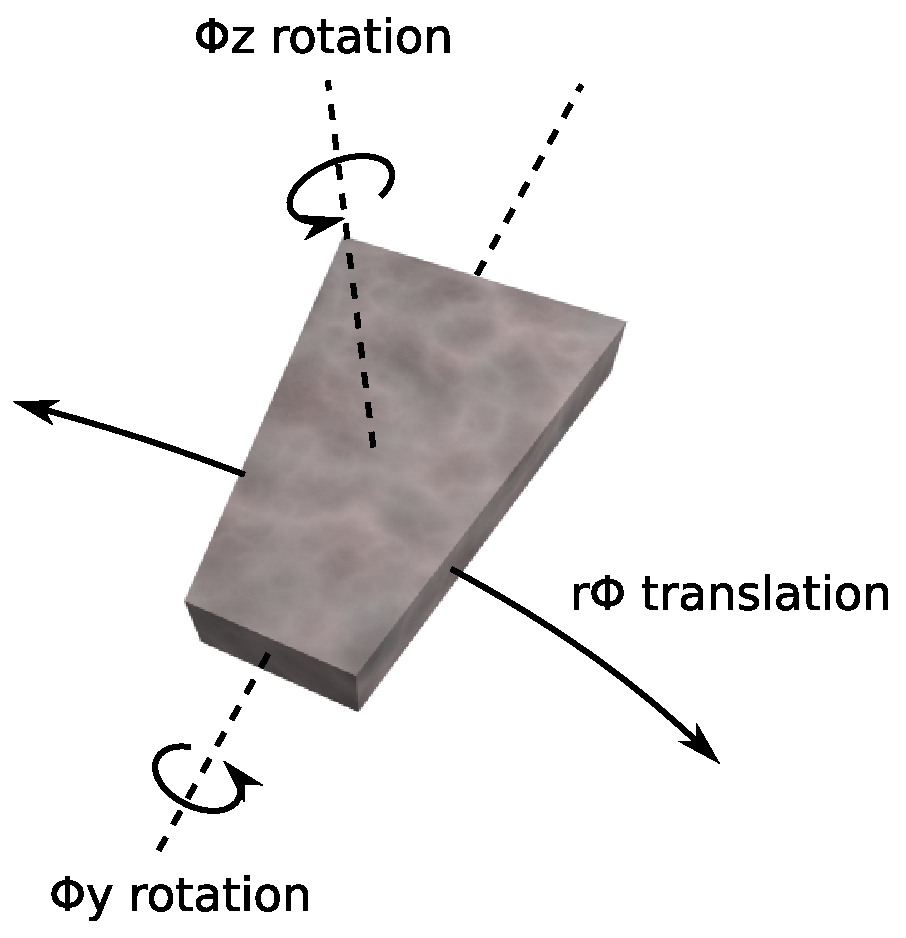
\includegraphics[width=0.5\linewidth]{csc_coordinates.eps}
\caption{Three aligned coordinates of CSC chambers.} \label{csc_coordinates}
\end{figure}

%%%%%%%%%%%%%%%%%%%%%%%%%%%%%%%%%%
\subsection{Monte Carlo simulation}

A Monte Carlo simulation approximating LHC beam-halo conditions was
used to test the procedure.  The simulation was not intended to model
the radial and azimuthal distribution of beam-halo muons from the LHC
exactly, as these are notoriously difficult to predict, but provided
a framework for testing the procedure with similar numbers of muons
($33\,000$ in the overlap regions).  Figure~\ref{mc_accuracy}
demonstrates that the alignment algorithm successfully restores the
correct alignment parameters from an initially misaligned system.

\begin{figure*}
\centering
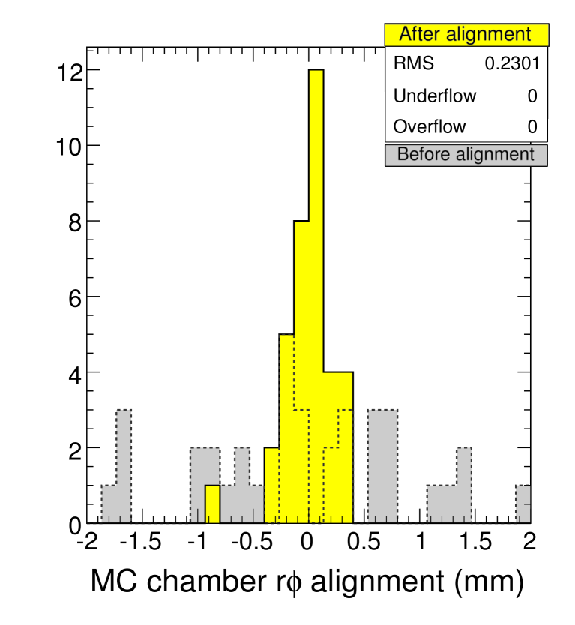
\includegraphics[width=0.32\linewidth]{mc_rphi.eps}
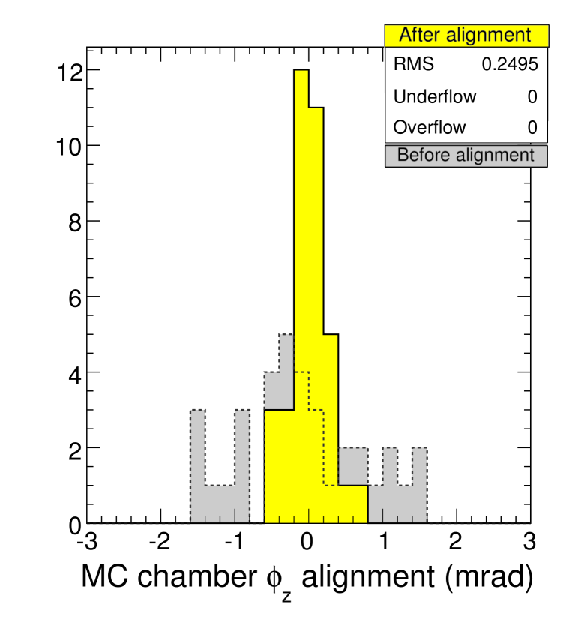
\includegraphics[width=0.32\linewidth]{mc_phiz.eps}
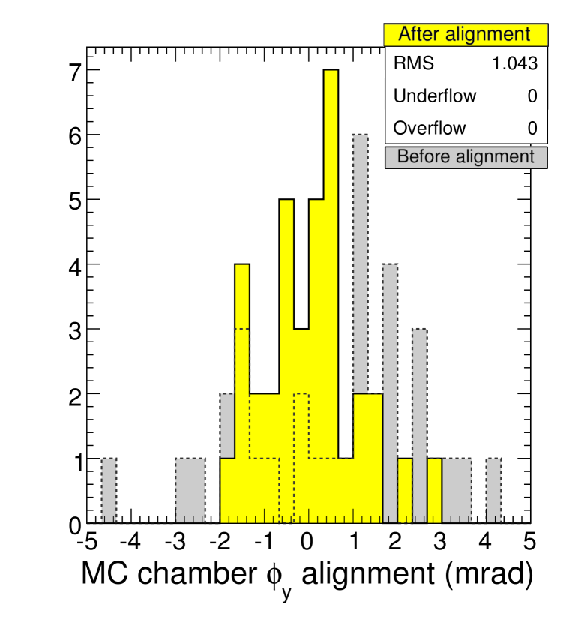
\includegraphics[width=0.32\linewidth]{mc_phiy.eps}
\caption{Histogram of aligned chamber parameters minus true chamber parameters for a simulated beam-halo alignment challenge.} \label{mc_accuracy}
\end{figure*}

%%%%%%%%%%%%%%%%%%%%%%%%%%%%%%%%%%
\subsection{Alignment cross-checks}

The alignment algorithm was applied using muons from the largest
beam-halo dataset: a 9-minute circulation of the anti-clockwise LHC
beam.  These muons primarily illuminated rings close to the beamline
and on the negative-$z$ side of CMS, so rings ME$-$2/1 and ME$-$3/1
were chosen for alignment.

An independent alignment was performed using photogrammetry
(measurement of photographs of the detector before it was fully
assembled), which we use to verify the track-based method.  In
Fig.~\ref{data_correlations}, differences between aligned and design
$\phi_z$ angles are plotted from the track-based method and
photogrammetry, in which we see a clear correlation.  These
comparisons are summarized by Fig.~\ref{data_accuracy}, in which
differences in $r\phi$ positions and $\phi_z$ angles (the two
parameters measurable by photogrammetry) between the two methods are
histogrammed.  Subtracting the photogrammetry uncertainty in
quadrature from the RMS of these histograms, the track-based accuracy
is 270~$\mu$m in $r\phi$ and 0.35~mrad in $\phi_z$--- on the scale of
the intrinsic hit resolutions (100--300~$\mu$m).

\begin{figure}
\centering
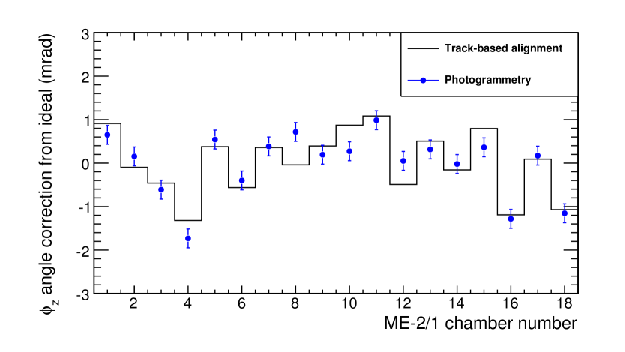
\includegraphics[width=0.9\linewidth]{data_correlations.eps}
\caption{Alignment corrections for a sample ring from the track-based method and from a photograph of the detector, illustrating a strong correlation.} \label{data_correlations}
\end{figure}

\begin{figure*}
\centering
\mbox{ } \hfill 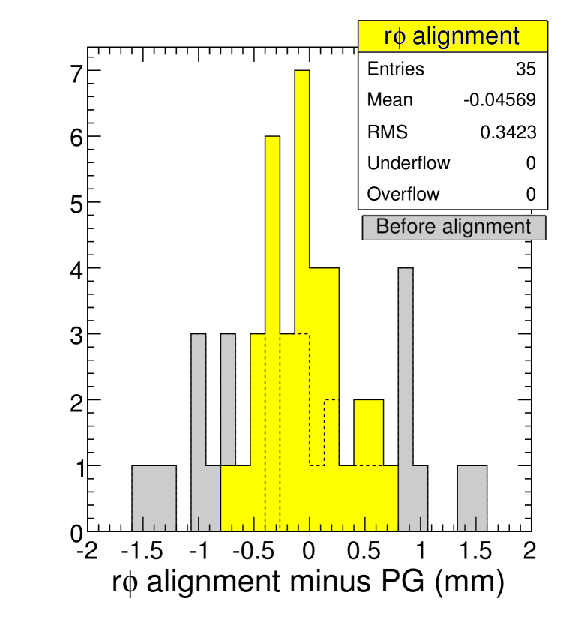
\includegraphics[width=0.35\linewidth]{data_rphi.eps} \hfill
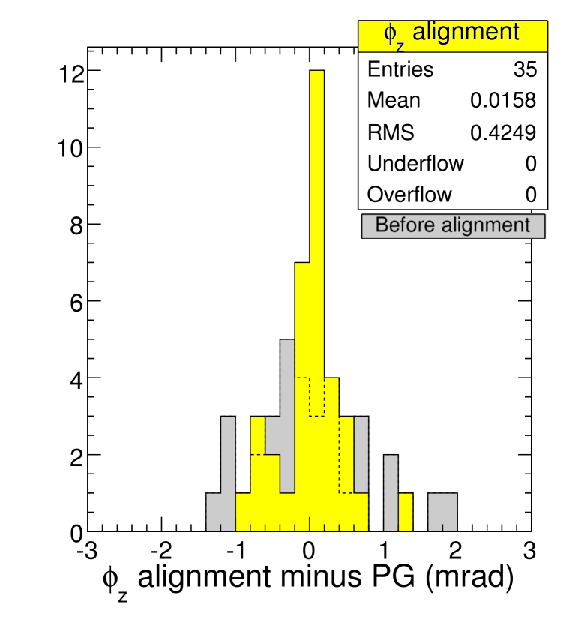
\includegraphics[width=0.35\linewidth]{data_phiz.eps} \hfill \mbox{ }
\caption{Histogram of aligned chamber parameters minus chamber parameters as measured by photogrammetry (PG).} \label{data_accuracy}
\end{figure*}

%%%%%%%%%%%%%%%%%%%%%%%%%%%%%%%%%%
\section{Conclusions}

Two track-based techniques were developed to align chambers in the CMS
muon system.  Both will be applied to muons from the first collisions
of the LHC, but they were first applied to available cosmic ray and
beam-halo data.  Alignment was shown to significantly improve the
momentum resolution of the central barrel DTs when aligned using
high-statistics cosmic rays, and independent methods of aligning the
inner-ring CSCs were shown to agree with high precision, despite the small
numbers of available tracks.  These tests demonstrate that CMS is
ready to achieve a precise alignment of the muon system when LHC
collisions become available, thereby optimizing high-energy muon
resolution for discoveries at the TeV energy scale.

%%%%%%%%%%%%%%%%%%%%%%%%%%%%%%%%%%
\begin{acknowledgments}
We thank the technical and administrative staff at CERN and other CMS
Institutes, and acknowledge support from: FMSR (Austria); FNRS and FWO
(Belgium); CNPq, CAPES, FAPERJ, and FAPESP (Brazil); MES (Bulgaria);
CERN; CAS, MoST, and NSFC (China); COLCIENCIAS (Colombia); MSES
(Croatia); RPF (Cyprus); Academy of Sciences and NICPB (Estonia);
Academy of Finland, ME, and HIP (Finland); CEA and CNRS/IN2P3
(France); BMBF, DFG, and HGF (Germany); GSRT (Greece); OTKA and NKTH
(Hungary); DAE and DST (India); IPM (Iran); SFI (Ireland); INFN
(Italy); NRF (Korea); LAS (Lithuania); CINVESTAV, CONACYT, SEP, and
UASLP-FAI (Mexico); PAEC (Pakistan); SCSR (Poland); FCT (Portugal);
JINR (Armenia, Belarus, Georgia, Ukraine, Uzbekistan); MST and MAE
(Russia); MSTDS (Serbia); MICINN and CPAN (Spain); Swiss Funding
Agencies (Switzerland); NSC (Taipei); TUBITAK and TAEK (Turkey); STFC
(United Kingdom); DOE and NSF (USA). Individuals have received support
from the Marie-Curie IEF program (European Union); the Leventis
Foundation; the A. P. Sloan Foundation; and the Alexander von Humboldt
Foundation.
\end{acknowledgments}

\bigskip % extra skip inserted
% Create the reference section using BibTeX:
%\bibliography{basename of .bib file}
\begin{thebibliography}{9}   % Use for  1-9  references
%\begin{thebibliography}{99} % Use for 10-99 references

\bibitem{cms} CMS Collaboration, ``The CMS Experiment at the CERN LHC,'' JINST {\bf 3} S08004, 2008.

\bibitem{lhc} L.~Evans and P.~Bryant (editors), ``LHC Machine,'' JINST {\bf 3} S08001, 2008.

\bibitem{mutdr} CMS Collaboration, ``Muon Technical Design Report,'' CERN-LHCC-97-32, 1997.

\end{thebibliography}

\end{document}
